\begin{abstract}
	Le dimensionnement de lots est un problème classique en planification de production. Différents critères \cite{cathy} permettent de classifier les problèmes de dimensionnement de lots. Suivant les classifications proposées, différentes classes peuvent être identifiées au nombre desquelles on peut citer le \emph{Discrete Lot Sizing Problem} (DLSP) dont le PSP fait partie. Différentes méthodes et modèles ont ainsi été appliqués au PSP \cite{ratheil_master} \cite{ceschia} avec différents résultats. Aussi, les algorithmes génétiques ont montré leur efficacité sur d'autres problèmes d'optimisation \cite{Goncalves}.
\end{abstract}

\section*{Introduction}
	\addcontentsline{toc}{section}{Introduction}
		
		Dans ce chapitre, nous présentons la revue de littérature des problèmes de dimensionnement de lots en planification de production dont fait parti le PSP. Nous exposons les méthodes de recherche déjà appliquées dans la résolution du PSP et soulignons les travaux effectués sur les algorithmes génétiques de même, nous montrons en quoi les algorithmes génétiques sont particulièrement adaptés à ces genres de problèmes.
		
	\section{Le dimensionnement de lots en planification de production}
	La planification de production est un processus qui consiste à déterminer un plan qui indique quelle quantité d'articles produire durant un intervalle de temps appelé "horizon de planification". Il est un important défi pour les entreprises industrielles car il a un fort impact sur leur performance en terme de qualité du service-client et des coûts d'exploitation. \\
	\hspace*{.5cm} Différentes recherches \cite{dauzere} ont été menées dans le but de classifier les problèmes de dimensionnement de lots. Plusieurs critères ont pu être identifiés. Nous présentons dans cette section quelques critères de classification \cite{cathy} des problèmes de dimensionnement de lots.
	
\subsection{Critères de classification}

Différents critères interviennent dans la classification des problèmes de dimensionnement de lots, notamment : 
\begin{description}
	\item[\textsl{L'échelle de temps}:] La planification peut être effectuée soit sur des périodes discrètes soit sur un horizon de temps continu. Dans le premier cas, la longueur des périodes peut être soit de petite taille (Small time buckets) correspondant à des heures ou jours, soit de grande taille (Big time buckets) correspondant à des jours ou semaines, soit de très grande taille (Very big time buckets) correspondant à des mois ou trimestres.

	\item[\textsl{Le nombre de niveaux}:] On distingue les problèmes à un niveau. Un état de l'art sur ce type de problème est proposé par Karimi et al. \cite{karimi} . Lorsqu'il existe une relation entre les produits, on considère des problèmes à plusieurs niveaux.

	\item[\textsl{Le nombre de produits}:] Dans le cas où il n'y a pas de dépendance entre les produits, en particulier, s'il n'y a pas d'utilisation commune de la capacité, nous considérons des problèmes à un seul produit. Dans le cas inverse, on parle de problèmes à plusieurs produits. Un état de l'art sur les problèmes à un produit est proposé par Brahimi et al. \cite{brahimi}.

	\item[\textsl{Les contraintes de capacité}:] Les contraintes de capacité incluent le nombre d'employés, la capacité des machines, la capacité de stockage, etc. Lorsque les contraintes de capacité sont
introduites dans le modèle, elles rendent le problème plus difficile à résoudre,
puisqu'elles lient les produits entre eux.

	\item[\textsl{Les demandes}:] Il existe plusieurs types de demandes qui peuvent être réparties selon trois
groupes :
	\begin{itemize}
		\item[•] les demandes constantes, les valeurs des demandes ne changent pas sur l'horizon de temps, ou demandes dynamiques , les valeurs varient au cours du temps.
		\item[•] les demandes certaines, les valeurs sont connues à l'avance, ou demandes stochastiques , les valeurs sont basées sur des probabilités.
		\item[•] les demandes indépendantes, lorsqu'un produit n'a pas besoin d'autres produits comme composants, ou demandes dépendantes, lorsqu'il existe une relation entre les produits.
	\end{itemize}

	\item[\textsl{Les coûts et temps de lancement ou préparation (setup)}:] Une ressource peut exécuter des produits de types différents. Ainsi, il est parfois nécessaire de reconfigurer celle-ci à chaque changement de produits. Les coûts et temps induits par le lancement de la ressource sont souvent importants car
élevés et longs.
	
\end{description}

	La complexité des problèmes de dimensionnement de lots varie fortement sous l'influence des différents facteurs comme le nombre de produits, le nombre de niveaux, les contraintes de capacité, etc. Nous avons choisi dans cette étude de décrire les problèmes de dimensionnement de lots selon la longueur de la période de l'horizon de temps. Nous allons donc nous intéresser aux problèmes à courtes et longues périodes.
\subsection{Classes de problèmes de dimensionnement de lots}
	\subsubsection{Problèmes à courtes périodes}
	Ces problèmes (\emph{Small time bucket problems}) sont caractérisés par des périodes de l'ordre de quelques heures, et la séquence des lots lors de la production est prise en compte. Quatre types de problèmes sont étudiés dans la littérature. Pour une étude détaillée de tous ces problèmes, nous pourrons nous référer à Drexl and Kimms \cite{drexl_kimms}. Ces différents types de problèmes sont donc:
	\begin{description}
		\item[\textsl{Discrete lot-sizing and scheduling problem :}]
		Ce problème noté DLSP, est initialement formulé par Fleischmann \cite{fleischmann}. La principale hypothèse de ce problème est qu'au plus un article peut être produit par
période. Si un article est fabriqué sur une période, alors toute la capacité disponible sur cette période sera utilisée. Généralement, les coûts de lancement sont pris en compte seulement lorsqu'un nouveau lot commence et non à chaque période.
		\item[\textsl{Continuous setup lot-sizing problem :}]
		Ce problème noté CSLP est similaire au précédent problème. La différence réside dans le fait que lorsqu'un article est produit sur une période, on utilise la capacité nécessaire pour produire cet article et non la capacité entière comme pour le problème précèdent.
		\item[\textsl{Proportional lot-sizing and scheduling problem : }] 
		Dans ce problème, que l'on notera PLSP, la capacité restante pour une période donnée est réutilisée pour produire un second article. Ce problème a été étudié par Drexl et Haase \cite{drexl_haase} et Kimms et Drexl \cite{drexl_kimms}. Il existe des extensions pour ce problème, par exemple, le cas à plusieurs niveaux et plusieurs machines. 
		\item[\textsl{General lot-sizing and scheduling problem : }] 
		Ce problème noté GLSP, est plus général que les problèmes précédents, puisque le nombre d'articles à produire par période n'est pas restrictif. Il est étudié par Fleischmann et Meyr \cite{fleischmann_meyr}. Il existe des extensions de ce problème, par exemple en intégrant des temps de lancement de production dépendant de la séquence des lots à produire (\cite{meyr}).
	\end{description}
	
	\subsubsection{Problèmes à longues périodes}
	Les problèmes à longues périodes (\emph{Big time bucket problems}) sont basés sur des
horizons de l'ordre de quelques jours à quelques semaines et sont caractérisés par le fait que plus d'un produit peut être fabriqué par période. Nous proposons dans cette section, une étude restreinte de ces problèmes.
	
	\begin{description}
		\item[Les problèmes à un niveau et un produit]: \\
		Ces problèmes ne correspondent pas vraiment à la réalité mais reçoivent beaucoup d'attention et d'intérêt puisque les méthodes mises en œuvre pour les résoudre sont généralisées dans le cas des problématiques à plusieurs niveaux.
		Les premiers travaux sur cette problématique ont été conduits par Manne \cite{manne}
et Wagner et Whitin \cite{wagner_whitin}. Leur méthode de résolution est utilisée dans plusieurs
concepts pour résoudre des problèmes plus complexes. Brahimi et al. \cite{brahimi} ont proposé
un état de l'art sur ces problématiques.		
		\item[Les problèmes à un niveau et plusieurs produits]: \\
		Le problème de dimensionnement de lots avec contraintes de capacité est considéré comme un problème complexe puisque la contrainte de capacité engendre un
lien entre les différents produits. Dans le cas où la capacité est considérée comme
infinie, le problème de dimensionnement de lots à N produits est réductible à N
problèmes à un produit et sans capacité, chacun solvable en temps polynomial.
		\item[Les problèmes à plusieurs niveaux]: \\ 
		Ces problèmes sont caractérisés par le fait que les produits finis sont fabriqués à partir de produits intermédiaires. Ainsi, les demandes dépendantes (i.e. les demandes entre les produits) et les demandes indépendantes (i.e. les demandes arrivant de l'extérieur) sont prises en compte dans ce type de problème.
	\end{description}
	
	Un exemple typique d'un problème de "\emph{big bucket}" est le "Capacited Lot Sizing Problem" (CLSP) , où différents articles peuvent être produit sur une même ressource en une seule période. Le CLSP classique consiste à déterminer le coût et le temps de production des articles dans l'horizon de planification: le résultat est un plan de production qui donne pour chaque période de planification, la quantité (\emph{lot size}) de chaque article qui doivent être produit. Le CLSP requiert que la ressource soit préparée pour un article donné dans la période où il est produit. La figure \ref{fig:classification_dimensionnement_lots} présente un exemple de classification des modèles de dimensionnement de lots.
	
	\begin{center}
		\begin{figure}[!h]
			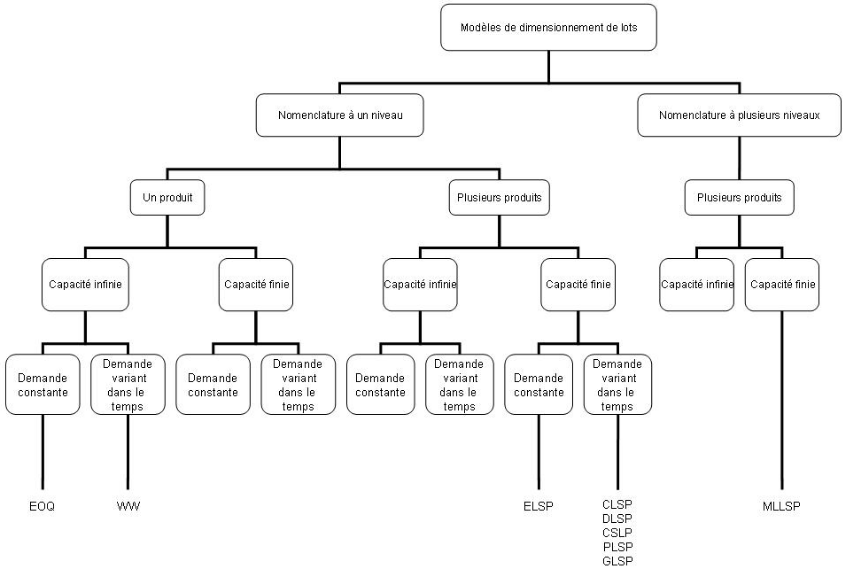
\includegraphics[scale=.5]{images/classification_dimensionnement.png}
			\caption{Exemple de classification des modèles de dimensionnement de lots \cite{cathy}}
			\label{fig:classification_dimensionnement_lots}
		\end{figure}
	\end{center}

	\newpage
	
	\section{Le \emph{Pigment sequencing problem} (PSP)}
	
	\subsection{Revue de littérature}
	Le PSP appartient à la catégorie des DLSP. En effet, il s'agit d'un problème où toute la capacité disponible sur cette période sera utilisée si un article est fabriqué. Nous présentons dans cette sous-section une brève revue de littérature des différents travaux effectués autour du PSP. \\
	\hspace*{.5cm} Miller et Wolsey \cite{miller_wolsey} ont formulé le DLSP avec des coûts de préparation indépendants de séquence comme un problème de réseau à flot. Ils ont présenté des formulations MIP pour les différentes extensions (avec \emph{backlogging}, avec stock de sûreté, avec stock initial). Plusieurs variantes et formulations MIP du DLSP ont été proposées et discutées par Pochet et Wolsey \cite{pochet_wolsey}. \\
	\hspace*{.5cm} Gicquel et al. \cite{gicquel_minoux_dallery} présentent une formulation et dérivent des inégalités valides pour le DLSP avec plusieurs articles et des coûts et temps de préparation séquentiels; laquelle est une extension du problème proposé par Wolsey \cite{wolsey}. Dans Gicquel et al. \cite {gicquel_miegeville_minoux_dallery}, les auteurs ont proposé une nouvelle manière de modéliser le DLSP avec plusieurs articles et des coûts et temps de préparation séquentiels; qui exploite le fait que les attributs physiques pertinents des articles, tels que la couleur, la dimension, le niveau de qualité. Cela leur a permis de réduire significativement le nombre des variables et des contraintes dans les modèles MIP.\\
	\hspace*{.5cm}Houndji et al. \cite{hvr_stockingCost} ont introduit une nouvelle contrainte globale, qu'ils ont appelée \emph{StockingCost} afin d'efficacement résoudre le PSP en programmation par contrainte. Les auteurs l'ont alors testée sur de nouvelles instances et les ont publiées sur CSPlib (Gent et Walsh \cite{gent_walsh}). Les résultats expérimentaux ont montré que le \emph{StockingCost} est plus efficace en filtrage tout en prenant en compte les autres techniques de décompositions généralement utilisées dans la communauté de la programmation par contrainte. \\
	\hspace*{.5cm} Plus récemment, Ceschia et al. \cite{ceschia} ont appliqué le recuit simulé sur le PSP. Ils ont implémenté une approche qui prend en charge à la fois la faisabilité de la solution et l'optimisation du coût. Dans le but d'illustrer leur méthode, ils ont introduit une procédure de recuit simulé afin de guider la recherche locale, qu'ils ont ensuite appliquée sur de nouvelles instances disponibles sur le bibliothèque Opthub \cite{opthub}.
	 
	\subsection{Description du problème}

		\label{sec:problem_description}
		Des différentes études \cite{ratheil_master} \cite{ceschia} déjà effectuées sur le PSP, nous pouvons le décrire comme une problème qui consiste à trouver un plan de production de plusieurs articles à partir d’une machine avec des coûts de transition. Les coûts de transition sont les coûts encourus lors du passage de la production de l’article $i$ à celui de l’article $j$ avec $i \neq j$. Le plan de production doit satisfaire les demandes des clients tout en :
	\begin{itemize}
		\item[•] respectant la capacité de production de la machine;
		\item[•] minimisant les coûts de stockage et de transition.
	\end{itemize}
	\hspace*{.5cm} On suppose que la période de production est suffisamment courte pour ne produire qu’au plus un article par période et que les demandes sont normalisées : la capacité de production de la machine est limitée à un article par
période et d($i$, $t$) $ \in $ {0, 1} avec $i$ l’article et $t$ la période.\\
	\hspace*{.5cm} Il s’agit d’un problème de planification de production ayant les caractéristiques suivantes : un horizon de planification discret et fini ; des contraintes de capacité ; une demande statique et déterministe ; multi-item et small bucket, des coûts de transition; un seul niveau; sans shortage.\\

	\textbf{\textsl{Illustration}} : Soit un problème avec les données ci-dessous : \\
	\begin{itemize}
		\item[•] Nombre d’articles : $NI = 2$;
		\item[•] Nombre de périodes : $NT = 5$;
		\item[•] Demande par période. Soit d($i$, $t$) la demande de l’article $i$ à la période $t$ : $d(1, t) = (0, 1, 0, 0, 1)$ et $d(2, t) = (1, 0, 0, 0, 1)$;
		\item[•] Coût de stockage. Soit $h(i)$ le coût de stockage de l’article $i$ : $h(1) = h(2) = 2$;
	\end{itemize}
	Soit \emph{xT} le plan de production qui représente une solution potentielle du problème. Il s’agit d’un tableau de dimension \emph{NT} , contenant à son indice $t$ (avec $t  \in  {1...NT}$) l’article $i$ à produire. Une solution admissible du problème est : $ xT = (2, 1, 2, 0, 1)$ avec un coût de $ q(2, 1) + q(1, 2) + q(2, 1) + 2 * h(2) = 15 $. La solution optimale est : $ xT = (2, 1, 0, 1, 2)$ avec un coût de $q(2, 1) + q(1, 2) + h(1) = 10$.
		
		\subsection{Modèles et formulations}
		Différents modèles ont été proposés afin de représenter, modéliser et résoudre le PSP. Il s'agit des modèles de programmation mixte en nombres entiers ou MIP (au nombre de 3) proposés par Pochet et Wolsey \cite{pochet_wolsey}, considérés comme l'état de l'art des méthodes de résolution exactes sur les problèmes de dimensionnement de lots en particulier celui du PSP, du modèle CP et du modèle SA. Nous présentons donc ici le premier modèle MIP dont les deux derniers sont une reformulation, le modèle CP ainsi que le modèle SA.
		\subsubsection{Modèle MIP 1}
		
		Le modèle MIP 1 \cite{pochet_wolsey} tel qu'exposé par Pochet et Wolsey se présente comme suit:
		\begin{eqnarray}
			min \sum_{i,j,t} q^{i,j}ch_{t}^{i,j} + \sum_{i,t} h^{i} s_{t}^{i} \\
			s_{0}^{i} = 0, \forall i \\
			x_{t}^{i} + s_{t-1}^{i} = d_{t}^{i} + s_{t}^{i}, \forall i,t \\
			x_{t}^{i} \leq y_{t}^{i}, \forall i,t \\
			\sum_{i} y_{t}^{i} = 1 , \forall t \\
			\chi_{t}^{i,j} = y_{t-1}^{i} + y_{t}^{j} - 1, \forall i,j,t \\
			x,y,\chi \in \{0,1\}, s \in N, i \in \{0..NI\}, t \in \{1..NT\}
		\end{eqnarray}
		
		avec les variables de décisions suivantes: \\
		\begin{itemize}
			\item[-] $x_{t}^{i}$ : variable binaire de production qui vaut 1 si l’article $i$ est produit à la période $t$ et 0 sinon ;
			\item[-] $y_{t}^{i}$ : variable binaire de setup qui vaut 1 si la machine est préparée pour la production de l’article $i$ et 0 sinon ;
			\item[-] $s_{t}^{i}$ : variable entière de stockage qui contient le nombre d’articles $i$ stockés à la période $t$ ; 
			\item[-] $\chi_{t}^{i,j}$ : variable binaire de transition qui vaut 1 si à la période $t$, on est passé de la production de l’article $i$ à l’article $j$ et 0 sinon.
		\end{itemize}
		\vspace*{.3cm}
	\hspace*{.5cm} L'objectif est de minimiser la somme des coûts de stockage et des coûts de transition et est exprimé par la contrainte (1). La contrainte (2) rappelle qu'il n'y a pas de stock initial. La contrainte (3) exprime la règle de la conservation de flot. La contrainte (4) vise à forcer la variable de setup $y_{t}^{i}$ à prendre la valeur 1 s’il y a production de l’article $i$ à la période $t$. La contrainte (5) s'assure qu'il y a toujours un article qui est préparé. En accord avec la fonction objectif, $y_{t}^{i}$ va prendre la valeur qui minimise le coût de transition. En général s’il n’y a pas de production à la période $t$,
$y_{t}^{i} = y_{t-1}^{i}$ ou $y_{t}^{i} = y_{t+1}^{i}$
mais parfois il peut être intéressant de préparer la machine pour un article intermédiaire sans le produire. La contrainte (6) assigne les valeurs aux variables de transition.
En effet, si $y_{t-1}^{i}$ et $y_{t}^{i}$ valent 1 alors $\chi_{t}^{i,j}$ est obligé de prendre la valeur 1 et sinon $ch_{t}^{i,j}$ serait égale à 0 grâce à la fonction objectif qui minimise le coût de transition.
		
		\subsubsection{Modèle CP}
		Dans ce modèle \cite{ratheil_master}, l’objectif est d’attribuer à chacune des demandes, une période qui respecte la date limite de satisfaction de la demande. On note $date(p) \in [1,...,T],\ \forall p \in [1,...,n]$ la période dans laquelle la demande $p$ a été satisfaite, $dueDate(p) \in [1,...,T]$ la date limite de la demande $p$ et $I(p)$ l'article correspondant à la demande $p$. Afin de s'assurer de la faisabilité de la solution, les principales contraintes sont les suivantes:
		\begin{eqnarray}
			date(p) \leq duedate(p), \forall p \\
			alldifferent(date)
		\end{eqnarray}
		
		dans lesquelles:
		\begin{itemize}
			\item[-] Equation 8: chaque demande doit être satisfaite avant sa date limite;
			\item[-] Equation 9: Puisque la capacité d'une machine est limitée à 1, chaque demande doit être satisfaite à différente période.
		\end{itemize}
		Il est possible de modeler la partie des coûts de transition comme un ATSP, chaque demande représente une ville qui doit être visitée et les coûts de transition sont les distances entre deux villes. Ainsi, on ajoute une demande artificielle $n+1$ de sorte que $date(n+1) = T+1$ avec $q^{I(p), I(n+1)} = q^{I(n+1), I(p)} = 0, \forall p \in [1,...,n]$. On note alors $successor(p), \forall p \in [1,...,n]$, la demande satisfaite juste après la satisfaction de la demande $p$. Les contraintes suivantes additionnelles peuvent être alors ajoutées:
		\begin{eqnarray}
			circuit(successor) \\
			date(p) \leq date(successor(p)), \forall p \in [1,...,n]
		\end{eqnarray}
		dans lesquelles:
		\begin{itemize}
			\item[-] Equation 10: il garantit l'existence d'un circuit hamiltonien;
			\item[-] Equation 11: la demande $p$ doit être satisfaite avant ses successeurs.
		\end{itemize}
		
		Enfin, l'objectif est de minimiser les coûts de stockage et les coûts de transition.
		\[
			\sum_{p}{(dueDate(p)-date(p))} * h_{I(p)} + \sum_{p}{q^{I(p),I(successor(p))}}
		\]
		
	
		\subsubsection{Modèle SA}
		Dans ce modèle \cite{ceschia}, la procédure de recuit simulé conduit à chaque itération à une action aléatoire en utilisant une distribution uniforme. Comme toujours en recuit simulé, l'action est toujours acceptée si elle est facteur d'amélioration. Dans le cas contraire, elle est acceptée, si elle est basée sur une distribution en temps croissant de façon exponentielle. Dans le détail, une mauvaise action est acceptée avec une probabilité de $e^{-\Delta/T}$ où $\Delta$ est la différence du coût total induit par l'action et $T$ est la température. La température commence à une valeur $T_{0}$ et est multipliée par $\alpha$ (avec $0 < \alpha < 1$), après un nombre fixé d'échantillons $n_{s}$, selon la procédure de refroidissement géométrique standard du recuit simulé. \\
		\hspace*{.5cm} Dans le but d'accélérer les premières étapes de la procédure de recuit simulé,  Ceschia et al. ont utilisé un mécanisme de \emph{cut-off} (Johnson et al. \cite{johnson}). Ils ont ajouté un nouveau paramètre $n_{a}$ représentant le nombre maximal d'actions acceptées à chaque niveau de température. Ainsi, la température diminue lorsque la première des deux conditions suivantes est remplie : ($i$) le nombre d'actions échantillonnées atteint $n_{s}$, ($ii$) le nombre d'actions acceptées atteint $n_{a}$. \\
		\hspace*{.5cm} Le critère de terminaison est basé sur le nombre total d'itérations $I_{max}$, plutôt que sur un seuil de température. De cette manière, le temps d'exécution est approximativement le même pour toutes les configurations des paramètres.
		
	\section{Les algorithmes génétiques}
		
	Les algorithmes génétiques (GAs) sont des algorithmes d’exploration fondés sur les mécanismes de la sélection naturelle et de la génétique \cite{holland1} \cite{holland2}. Ils utilisent à la fois les principes de la survie des structures les mieux adaptées, et les échanges d’informations aléatoires, parfois guidés, pour former un algorithme d’exploration qui possède certaines des caractéristiques de l’exploration humaine. Ils ont été proposés pour la première fois et sont devenues populaires à travers les travaux de John Holland au début des années 1970, et particulièrement son livre \emph{Adapation in Natural an Artificial Systems} (1975). Holland présenta les GAs comme une abstraction de l'évolution biologique et des concepts théoriques à l'adaptation pour les GAs dans son livre. Il introduisit un formalisme afin de prédire la qualité de la prochaine génération, plus connue comme le théorème des schémas de Holland.
	
	\subsection{Concepts de base}
	Les AGs constituent une classe de stratégies de recherche réalisant un compromis entre l’exploration et l’exploitation. Ils représentent des méthodes qui utilisent
un choix aléatoire comme outil pour guider une exploration intelligente dans l’espace des paramètres codés. Ce sont des algorithmes itératifs de recherche globale dont l’objectif est d’optimiser une fonction prédéfinie appelée fonction coût ou fonction « fitness ».
	Les algorithmes génétiques emploient un vocabulaire emprunté à la génétique naturelle. Ils travaillent sur un ensemble d’individus appelé population. Un individu a deux représentations appelées phénotype et génotype. Le phénotype représente une solution potentielle du problème à optimiser en utilisant la formulation originale du problème. Le génotype donne une représentation codée
d’une solution potentielle sous la forme d’un chromosome. Un chromosome est formé de gènes disposés en une succession linéaire et chaque gène peut prendre plusieurs
valeurs appelées allèles. Par exemple, un chromosome se compose d’une succession de 0 et de 1 (c.-à-d. une chaîne binaire), et la valeur pour une certaine position correspond à "on" (la valeur = 1) ou à "off" (la valeur = 0) d’un certain dispositif. Des formes plus compliquées, telles qu’un ordre des symboles et une permutation des alphabets, sont choisies pour décrire les chromosomes du problème à optimiser. Chaque individu a une fonction objectif f (fonction « fitness ») qui mesure l’adaptation de l’individu à son environnement local. La théorie darwinienne indique que, parmi des individus d’une population, celui qui est le mieux adapté à l’environnement local a le plus de chance de survivre et d’avoir un plus grand nombre de descendants : c’est la règle de la « survie du plus fort ». Ainsi, la
fonction objectif f du problème d’optimisation joue le rôle d’un critère d’adaptation. Un des points les plus importants des algorithmes génétiques est la flexibilité dans la fonction objectif.

	\subsection{Fonctionnement}
	
	L'algorithme \ref{algo:algo_genetique_standard} présente le principe de fonctionnement de l'algorithme génétique simple.\\
	 
	\begin{algorithm}[H]
 	\caption{Algorithme génétique standard \cite{Goncalves}}
 	\label{algo:algo_genetique_standard}
 	%\KwData{this text}
 	%\KwResult{how to write algorithm with \LaTeX2e }
 	%initialization\;
 	Générer la population initiale $P_{i}$ \\
 	Évaluer la population $P_{i}$ \\
 	\While{le critère de terminaison n'est pas satisfait}{
 	 Sélectionner les éléments de $P_{i}$ à copier dans $P_{i+1}$ \\
 	 Appliquer le croisement aux éléments de $P_{i}$ et les mettre dans $P_{i+1}$ \\
 	 Appliquer la mutation aux éléments de $P_{i}$ et les mettre dans $P_{i+1}$ \\
 	 Évaluer la nouvelle population $P_{i+1}$ \\
 	 $P_{i}$ = $P_{i+1}$
 	}
	\end{algorithm}
	
	\vspace*{1cm}
	Cet algorithme \ref{algo:algo_genetique_standard} est explicité plus en détails à l'aide de la figure \ref{fig:genetic_algo_flowchart}.
	
	\begin{figure}[!h]
		\begin{center}
			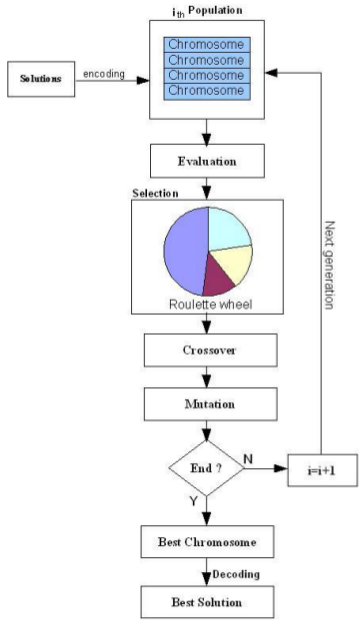
\includegraphics[scale=.5]{images/genetic_algo_flowchart.png}
			\caption{Diagramme d'un algorithme génétique standard \cite{denny}}
			\label{fig:genetic_algo_flowchart}
		\end{center}
	\end{figure}
	
	\newpage
	
	\subsection{Les opérateurs}
		Un algorithme génétique simple utilise les trois opérateurs suivants : la sélection, le croisement et la mutation.
		\subsubsection{L’opérateur de sélection}
		La sélection est un processus dans lequel des individus d’une population sont choisis selon les valeurs de leur fonction coût ou «  fitness  » pour former une nouvelle population. Les individus évoluent par des itérations successives de la sélection, appelées générations. Chaque individu est sélectionné proportionnellement à sa fonction « fitness », donc, un individu avec une fonction « fitness »
plus élevée aura plus de chance d’être sélectionné qu’un autre avec une valeur de « fitness » inférieure. Cette fonction peut être envisagée comme une mesure de profit ou de qualité qu’on souhaite maximiser. Un opérateur simple de sélection est la technique de la roulette pondérée où chaque individu d’une population
occupe une surface de la roulette proportionnelle à la valeur de sa fonction « fitness ». Pour la reproduction, les candidats sont sélectionnés avec une probabilité proportionnelle à leur «  fitness  ». Pour chaque sélection d’un
individu, une simple rotation de la roue donne le candidat sélectionné. Cependant cette sélection n’est pas parfaite. En effet, le risque de favoriser un individu ou un petit ensemble d’individus constitue un inconvénient qui risque d’appauvrir la diversité de la population.
	\subsubsection{L’opérateur de croisement}
	Le croisement est un opérateur de recombinaison. Les individus d’une population sont couplés au hasard par paires représentant les parents. Chaque paire d’individus
subit le croisement décrit comme suit : le croisement opère sur les génotypes (c.-à-d. les chromosomes) de deux individus appelés parents. Il produit de nouveaux individus (généralement deux) appelés enfants dont les gènes sont hérités de l’un ou/et de l’autre parent. Ceci peut être fait en dédoublant chacun des deux chromosomes dans des fragments et en les recombinant pour former de nouveaux chromosomes.
	\begin{description}
		\item[\textsl{Le croisement à un point :}] Si le génotype est une chaîne binaire de longueur n. Le croisement à un point place un point de croisement au
hasard. Un enfant prend une section avant le point de croisement d’un parent et prend l’autre section après le point de croisement de l’autre parent puis recombine les deux sections pour former une nouvelle chaîne binaire. L’autre enfant se construit inversement. 
		
		\item[\textsl{Le croisement à deux points :}]Le croisement à deux points place deux points de croisement au hasard, et prend une section entre les points d’un parent et les autres sections en dehors des points de l’autre parent puis les recombine. 
	
		\item[\textsl{Le croisement uniforme :}]Ce type de croisement a été proposé par Syswerda \cite{Syswerda}. Il consiste à choisir avec la même probabilité un allèle de l’un ou de l’autre parent, pour transmettre sa valeur à la même position, aux enfants. 
	
	\end{description}
	
	\subsubsection{L'opérateur de mutation}
	
	La mutation opère sur le génotype d’un seul individu. Elle correspond, dans la nature, à une « erreur » qui se produit quand le chromosome est copié et reproduit. Dans une approche numérique, pour une chaîne binaire, elle consiste par exemple à faire pour un allèle un échange entre le « 0 » et le « 1 ». Si des copies exactes sont toujours garanties, alors le taux de mutation est égal à zéro. Cependant, dans la vie réelle, l’erreur de copie peut se produire dans diverses circonstances comme sous l’influence d’un bruit. La mutation change les valeurs de certains gènes avec une faible probabilité. Elle n’améliore pas, en général, les solutions, mais elle évite une perte irréparable de la diversité.
	
	\subsection{Application des algorithmes génétiques aux problèmes d'optimisation}
	
	Les algorithmes génétiques ont été largement utilisées ces dernières années \cite{jawahar}. L’utilisation des AGs dans de nombreux domaines a fait ses preuves, notamment dans des problèmes combinatoires tels que les problèmes d’ordonnancement \cite{davis} et les problèmes de collecte et de distribution. Les problèmes d’ordonnancement d’un atelier classique de type Job-Shop (JSP) ont notamment été largement étudiés et résolus par les AGs \cite{boukef}. D’autres algorithmes hybrides ont été aussi proposés \cite{cavalieri}. La difficulté principale dans la résolution de ces types de problèmes résulte dans la façon avec laquelle ils sont représentés sous forme algorithmique. Dans cette phase, la définition du chromosome représente le point le plus important dans la recherche génétique. Plusieurs approches de représentation et différents types d’opérateurs d’AGs ont été proposés, pour résoudre ces problèmes.
	
	\section*{Conclusion}
	\addcontentsline{toc}{section}{Conclusion}
	Le dimensionnement de lots en planification de production est un important défi pour les entreprises industrielles. Il consiste à trouver un plan de production qui satisfait aux contraintes spécifiques relatives au système de production. Le PSP constitue en effet une variante NP-Difficile de ces types de problèmes. Plusieurs méthodes peuvent servir à résoudre ce problème. Au nombre de ces méthodes, figurent les algorithmes génétiques. Les AGs, à travers l'exploration et l'exploitation de l'espace de recherche ont permis de résoudre bon nombre de problèmes d'optimisation par le passé. Nous avons également présenté le PSP ainsi que les modèles et leur formulation qui ont été utilisés dans sa résolution.	Dans le partie suivante, nous décrivons les outils de test, les méthodes de résolution proposées ainsi que les algorithmes associés.
